\documentclass{beamer}
\setbeamertemplate{navigation symbols}{}

\usepackage{tikz}
\usepackage{listings}

\usetheme{Warsaw}

\beamersetuncovermixins{\opaqueness<1>{25}}{\opaqueness<2->{15}}
\begin{document}
\title{LexBFS and its applications}  
\author{Guillaume Aubian}
\date{\today} 


\begin{frame}
\titlepage
\end{frame}

\begin{frame}\frametitle{Overview}\tableofcontents
\end{frame} 


\begin{frame}\frametitle{Before we start : a small sidequest}
     \Huge
	\textbf{Input :} a graph $G$

     	\textbf{Output :} a BFS on $\bar{G}$
     
     	\textbf{Time complexity :} linear
\end{frame}

\begin{frame}\frametitle{What's in a graph ?}
    \begin{block}{Graph}
	We consider non-oriented, simple and \textbf{connected} graphs
    \end{block}

    \begin{center}
    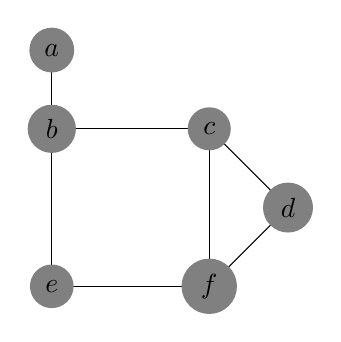
\begin{tikzpicture}  

	\draw (0,0) -- (0,2);
	\draw (0,0) -- (2,0);
	\draw (2,2) -- (0,2);
	\draw (2,2) -- (2,0);
	\draw (2,2) -- (3,1);
	\draw (2,0) -- (3,1);
	\draw (0,2) -- (0,3);

	\draw (0,0) node[circle, fill=gray]{$e$} ;
	\draw (2,0) node[circle, fill=gray]{$f$} ;
	\draw (0,2) node[circle, fill=gray]{$b$} ;
	\draw (2,2) node[circle, fill=gray]{$c$} ;
	\draw (3,1) node[circle, fill=gray]{$d$} ;
	\draw (0,3) node[circle, fill=gray]{$a$} ;


    \end{tikzpicture}
    \end{center}

\end{frame}

\begin{frame}[fragile]\frametitle{Generic Search}
    \begin{lstlisting}[language = Python]
    for i in [1, ..., n]:
        if i == 1:
	    u = any vertex
	else:
	    u = any unvisited marked vertex
	visit(u)
	for v in neighbours(u):
	    mark(v)
    \end{lstlisting}
\end{frame}

\begin{frame}\frametitle{Example of generic search}
    \begin{center}
    \begin{tikzpicture}  

	\draw (0,0) -- (0,2);
	\draw (0,0) -- (2,0);
	\draw (2,2) -- (0,2);
	\draw (2,2) -- (2,0);
	\draw (2,2) -- (3,1);
	\draw (2,0) -- (3,1);
	\draw (0,2) -- (0,3);

	\draw (0,0) node[circle, fill=gray]{$e$} ;
	\draw (2,0) node[circle, fill=gray]{$f$} ;
	\draw (0,2) node[circle, fill=gray]{$b$} ;
	\draw (2,2) node[circle, fill=gray]{$c$} ;
	\draw (3,1) node[circle, fill=gray]{$d$} ;
	\draw (0,3) node[circle, fill=gray]{$a$} ;

	\only<1-6>{
	\draw (0,0) node[circle, fill=orange]{$e$} ;
	}
	\only<3-6>{
	\draw (0,0) node[circle, fill=red]{$e$} ;
	}

	\only<1-6>{
	\draw (2,0) node[circle, fill=red]{$f$} ;
	}

	\only<2-6>{
	\draw (0,2) node[circle, fill=orange]{$b$} ;
	}
	\only<4-6>{
	\draw (0,2) node[circle, fill=red]{$b$} ;

	}

	\only<1-6>{
	\draw (2,2) node[circle, fill=orange]{$c$} ;
	}
	\only<2-6>{
	\draw (2,2) node[circle, fill=red]{$c$} ;
	}

	\only<1-6>{
	\draw (3,1) node[circle, fill=orange]{$d$} ;
	}
	\only<5-6>{
	\draw (3,1) node[circle, fill=red]{$d$} ;
	}

	\only<4-6>{
	\draw (0,3) node[circle, fill=orange]{$a$} ;
	}
	\only<6-6>{
	\draw (0,3) node[circle, fill=red]{$a$} ;
	}

    \end{tikzpicture}
    \end{center}

\end{frame}

\begin{frame}\frametitle{Another Characterization}
    Let's number vertices in the order they are visited.
    \begin{theorem}
        An ordering $\sigma$ corresponds to a Generic Search if and only if
	    
	    $$\forall a <_{\sigma} b <_{\sigma} c, ac \in E\text{ and }ab \notin E, \exists d <_{\sigma} b\text{ st }db \in E$$
    \end{theorem}
    \begin{center}
    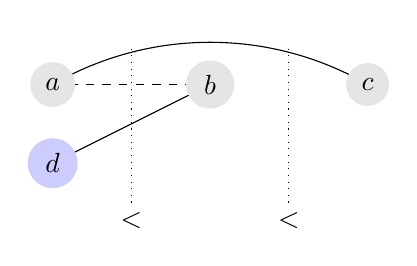
\begin{tikzpicture}  

	\draw (0,1) arc (120:60:4) ;
	\draw [dashed] (0,1) -- (2,1);
	\draw (0,0) -- (2,1);
	\draw (0,0) node[circle, fill=blue!20]{$d$} ;
	\draw (0,1) node[circle, fill=gray!20]{$a$} ;
	\draw (2,1) node[circle, fill=gray!20]{$b$} ;
	\draw (4,1) node[circle, fill=gray!20]{$c$} ;


	\draw [dotted] (1,-0.5) -- (1,1.5);
	\draw [dotted] (3,-0.5) -- (3,1.5);
	\draw (1,-0.5) node[below]{$<$} ;
	\draw (3,-0.5) node[below]{$<$} ;
    \end{tikzpicture}
    \end{center}
\end{frame}




\begin{frame}[fragile]\frametitle{DFS}
    \begin{lstlisting}[language = Python]
    for i in [1, ..., n]:
        if i == 1:
	    u = any vertex
	else:
	    u = any unvisited vertex w/ max label
	visit(u)
	for v in neighbours(u):
	    label[v] = i
    \end{lstlisting}
\end{frame}

\begin{frame}[fragile]\frametitle{DFS example}
    \begin{center}
    \begin{tikzpicture}  

	\draw (0,0) -- (0,2);
	\draw (0,0) -- (2,0);
	\draw (2,2) -- (0,2);
	\draw (2,2) -- (2,0);
	\draw (2,2) -- (3,1);
	\draw (2,0) -- (3,1);
	\draw (0,2) -- (0,3);

	\draw (0,0) node[circle, fill=gray]{$e$} ;
	\draw (2,0) node[circle, fill=gray]{$f$} ;
	\draw (0,2) node[circle, fill=gray]{$b$} ;
	\draw (2,2) node[circle, fill=gray]{$c$} ;
	\draw (3,1) node[circle, fill=gray]{$d$} ;
	\draw (0,3) node[circle, fill=gray]{$a$} ;

	\only<1-6>{
	\draw (0,0) node[circle, fill=orange]{$e$} ;
	}
	\only<5-6>{
	\draw (0,0) node[circle, fill=red]{$e$} ;
	}

	\only<1-6>{
	\draw (2,0) node[circle, fill=red]{$f$} ;
	}

	\only<3-6>{
	\draw (0,2) node[circle, fill=orange]{$b$} ;
	}
	\only<4-6>{
	\draw (0,2) node[circle, fill=red]{$b$} ;

	}

	\only<1-6>{
	\draw (2,2) node[circle, fill=orange]{$c$} ;
	}
	\only<3-6>{
	\draw (2,2) node[circle, fill=red]{$c$} ;
	}

	\only<1-6>{
	\draw (3,1) node[circle, fill=orange]{$d$} ;
	}
	\only<2-6>{
	\draw (3,1) node[circle, fill=red]{$d$} ;
	}

	\only<4-6>{
	\draw (0,3) node[circle, fill=orange]{$a$} ;
	}
	\only<6-6>{
	\draw (0,3) node[circle, fill=red]{$a$} ;
	}

    \end{tikzpicture}
    \end{center}
\end{frame}



\begin{frame}\frametitle{Another Characterization}
    \begin{theorem}
        An ordering $\sigma$ corresponds to a DFS if and only if
	    
	    $$\forall a <_{\sigma} b <_{\sigma} c, ac \in E\text{ and }ab \notin E, \exists a <_{\sigma} d <_{\sigma} b\text{ st }db \in E$$
    \end{theorem}
    \begin{center}
    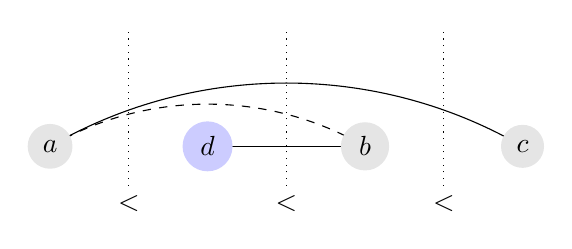
\begin{tikzpicture}
	\draw (0,0) arc (120:60:6) ;
	\draw (2,0) -- (4,0);
	\draw [dashed] (0,0) arc (120:60:4) ;

	\draw (0,0) node[circle, fill=gray!20]{$a$} ;
	\draw (2,0) node[circle, fill=blue!20]{$d$} ;
	\draw (4,0) node[circle, fill=gray!20]{$b$} ;
	\draw (6,0) node[circle, fill=gray!20]{$c$} ;




	\draw [dotted] (1,-0.5) -- (1,1.5);
	\draw [dotted] (3,-0.5) -- (3,1.5);
	\draw [dotted] (5,-0.5) -- (5,1.5);

	\draw (1,-0.5) node[below]{$<$} ;
	\draw (3,-0.5) node[below]{$<$} ;
	\draw (5,-0.5) node[below]{$<$} ;
    \end{tikzpicture}
    \end{center}

\end{frame}


\begin{frame}[fragile]\frametitle{BFS}
    \begin{lstlisting}[language = Python]
    for i in [n, ..., 1]:
        if i == n:
	    u = any vertex
	else:
	    u = any unvisited vertex w/ max label
	visit(u)
	for v in neighbours(u):
	    if v has no label:
	        label[v] = i
    \end{lstlisting}
\end{frame}


\begin{frame}[fragile]\frametitle{BFS example}

    \begin{center}
    \begin{tikzpicture}  

	\draw (0,0) -- (0,2);
	\draw (0,0) -- (2,0);
	\draw (2,2) -- (0,2);
	\draw (2,2) -- (2,0);
	\draw (2,2) -- (3,1);
	\draw (2,0) -- (3,1);
	\draw (0,2) -- (0,3);

	\draw (0,0) node[circle, fill=gray]{$e$} ;
	\draw (2,0) node[circle, fill=gray]{$f$} ;
	\draw (0,2) node[circle, fill=gray]{$b$} ;
	\draw (2,2) node[circle, fill=gray]{$c$} ;
	\draw (3,1) node[circle, fill=gray]{$d$} ;
	\draw (0,3) node[circle, fill=gray]{$a$} ;

	\only<1-6>{
	\draw (0,0) node[circle, fill=orange]{$e$} ;
	}
	\only<4-6>{
	\draw (0,0) node[circle, fill=red]{$e$} ;
	}

	\only<1-6>{
	\draw (2,0) node[circle, fill=red]{$f$} ;
	}

	\only<3-6>{
	\draw (0,2) node[circle, fill=orange]{$b$} ;
	}
	\only<5-6>{
	\draw (0,2) node[circle, fill=red]{$b$} ;

	}

	\only<1-6>{
	\draw (2,2) node[circle, fill=orange]{$c$} ;
	}
	\only<3-6>{
	\draw (2,2) node[circle, fill=red]{$c$} ;
	}

	\only<1-6>{
	\draw (3,1) node[circle, fill=orange]{$d$} ;
	}
	\only<2-6>{
	\draw (3,1) node[circle, fill=red]{$d$} ;
	}

	\only<5-6>{
	\draw (0,3) node[circle, fill=orange]{$a$} ;
	}
	\only<6-6>{
	\draw (0,3) node[circle, fill=red]{$a$} ;
	}

    \end{tikzpicture}
    \end{center}


\end{frame}


\begin{frame}\frametitle{Another Characterization}
    \begin{theorem}
        An ordering $\sigma$ corresponds to a BFS if and only if
	    
	    $$\forall a <_{\sigma} b <_{\sigma} c, ac \in E\text{ and }ab \notin E, \exists d <_{\sigma} a\text{ st }db \in E$$
    \end{theorem}

    \begin{center}
    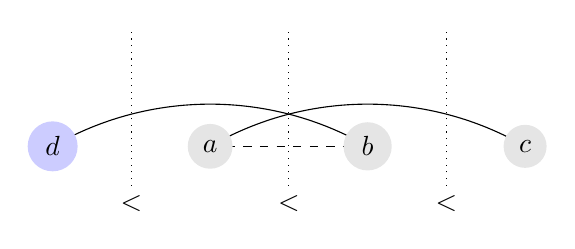
\begin{tikzpicture}
	\draw (0,0) arc (120:60:4) ;
	\draw (2,0) arc (120:60:4) ;
	\draw [dashed] (2,0) -- (4,0);

	\draw (0,0) node[circle, fill=blue!20]{$d$} ;
	\draw (2,0) node[circle, fill=gray!20]{$a$} ;
	\draw (4,0) node[circle, fill=gray!20]{$b$} ;
	\draw (6,0) node[circle, fill=gray!20]{$c$} ;

	\draw [dotted] (1,-0.5) -- (1,1.5);
	\draw [dotted] (3,-0.5) -- (3,1.5);
	\draw [dotted] (5,-0.5) -- (5,1.5);

	\draw (1,-0.5) node[below]{$<$} ;
	\draw (3,-0.5) node[below]{$<$} ;
	\draw (5,-0.5) node[below]{$<$} ;
    \end{tikzpicture}
    \end{center}

\end{frame}

\begin{frame}[fragile]\frametitle{Let's rewrite BFS}
    \begin{lstlisting}[language = Python]
    for i in [n, ..., 1]:
        if i == n:
	    u = any vertex
	else:
	    u = any unvisited vertex
	        w/ max first element of label
	visit(u)
	for v in neighbours(u):
	    label[v].append(i)
    \end{lstlisting}
\end{frame}

\begin{frame}[fragile]\frametitle{Here is LexBFS}
    \begin{lstlisting}[language = Python]
    for i in [n, ..., 1]:
        if i == n:
	    u = any vertex
	else:
	    u = any unvisited vertex
	        w/ max lexicographical label
	visit(u)
	for v in neighbours(u):
	    label[v].append(i)
    \end{lstlisting}
\end{frame}

\begin{frame}[fragile]\frametitle{LexBFS example}

    \begin{center}
    \begin{tikzpicture}  

	\draw (0,0) -- (0,2);
	\draw (0,0) -- (2,0);
	\draw (2,2) -- (0,2);
	\draw (2,2) -- (2,0);
	\draw (2,2) -- (3,1);
	\draw (2,0) -- (3,1);
	\draw (0,2) -- (0,3);

	\draw (0,0) node[circle, fill=gray]{$e$} ;
	\draw (2,0) node[circle, fill=gray]{$f$} ;
	\draw (0,2) node[circle, fill=gray]{$b$} ;
	\draw (2,2) node[circle, fill=gray]{$c$} ;
	\draw (3,1) node[circle, fill=gray]{$d$} ;
	\draw (0,3) node[circle, fill=gray]{$a$} ;

	\only<1-6>{
	\draw (0,0) node[circle, fill=orange]{$e$} ;
	}
	\only<4-6>{
	\draw (0,0) node[circle, fill=red]{$e$} ;
	}

	\only<1-6>{
	\draw (2,0) node[circle, fill=red]{$f$} ;
	}

	\only<3-6>{
	\draw (0,2) node[circle, fill=orange]{$b$} ;
	}
	\only<5-6>{
	\draw (0,2) node[circle, fill=red]{$b$} ;

	}

	\only<1-6>{
	\draw (2,2) node[circle, fill=orange]{$c$} ;
	}
	\only<3-6>{
	\draw (2,2) node[circle, fill=red]{$c$} ;
	}

	\only<1-6>{
	\draw (3,1) node[circle, fill=orange]{$d$} ;
	}
	\only<2-6>{
	\draw (3,1) node[circle, fill=red]{$d$} ;
	}

	\only<5-6>{
	\draw (0,3) node[circle, fill=orange]{$a$} ;
	}
	\only<6-6>{
	\draw (0,3) node[circle, fill=red]{$a$} ;
	}

    \end{tikzpicture}
    \end{center}


\end{frame}



\begin{frame}\frametitle{Another Characterization}
    \begin{theorem}
        An ordering $\sigma$ corresponds to a LexBFS if and only if
	    
	    $$\forall a <_{\sigma} b <_{\sigma} c, ac \in E\text{ and }ab \notin E, \exists d <_{\sigma} a\text{ st }db \in E\text{ and }dc \notin E$$
	 
    \end{theorem}

    \begin{center}
    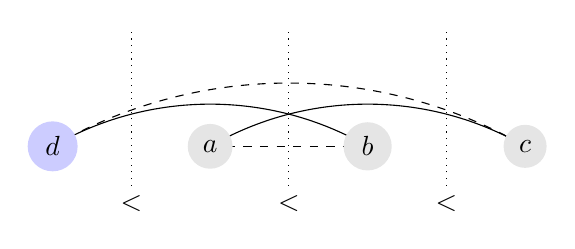
\begin{tikzpicture}
	\draw (0,0) arc (120:60:4) ;
	\draw (2,0) arc (120:60:4) ;
	\draw [dashed] (2,0) -- (4,0);
	\draw [dashed] (0,0) arc (120:60:6) ;

	\draw (0,0) node[circle, fill=blue!20]{$d$} ;
	\draw (2,0) node[circle, fill=gray!20]{$a$} ;
	\draw (4,0) node[circle, fill=gray!20]{$b$} ;
	\draw (6,0) node[circle, fill=gray!20]{$c$} ;


	\draw [dotted] (1,-0.5) -- (1,1.5);
	\draw [dotted] (3,-0.5) -- (3,1.5);
	\draw [dotted] (5,-0.5) -- (5,1.5);

	\draw (1,-0.5) node[below]{$<$} ;
	\draw (3,-0.5) node[below]{$<$} ;
	\draw (5,-0.5) node[below]{$<$} ;
    \end{tikzpicture}
    \end{center}
\end{frame}

\begin{frame}\frametitle{Another Characterization}
    Iterating on [1, ..., n] and prepending, we obtain LexDFS
    \begin{theorem}
        An ordering $\sigma$ corresponds to a LexDFS if and only if
	    
	    $$\forall a <_{\sigma} b <_{\sigma} c, ac \in E, ab \notin E, \exists a <_{\sigma} d <_{\sigma} b\text{ st }db \in E, dc \notin E$$
    \end{theorem}
    \begin{center}
    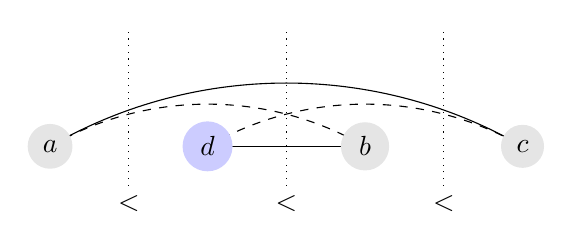
\begin{tikzpicture}
	\draw (0,0) arc (120:60:6) ;
	\draw (2,0) -- (4,0);
	\draw [dashed] (0,0) arc (120:60:4) ;
	\draw [dashed] (2,0) arc (120:60:4) ;

	\draw (0,0) node[circle, fill=gray!20]{$a$} ;
	\draw (2,0) node[circle, fill=blue!20]{$d$} ;
	\draw (4,0) node[circle, fill=gray!20]{$b$} ;
	\draw (6,0) node[circle, fill=gray!20]{$c$} ;

	\draw [dotted] (1,-0.5) -- (1,1.5);
	\draw [dotted] (3,-0.5) -- (3,1.5);
	\draw [dotted] (5,-0.5) -- (5,1.5);

	\draw (1,-0.5) node[below]{$<$} ;
	\draw (3,-0.5) node[below]{$<$} ;
	\draw (5,-0.5) node[below]{$<$} ;
    \end{tikzpicture}
    \end{center}
\end{frame}

\begin{frame}\frametitle{How to implement LexBFS: Pivoting}
    \only<1>{Let's order vertices by label :}
    \only<2>{We remove one of the maximum vertex :}
    \only<3>{Now, we split each bucket}
    \only<1-2>{
    \begin{center}
    \begin{tikzpicture}
	\draw (0,-2) node[circle, fill=black]{} ;
	\draw (0,0) node[circle, fill=black]{} ;
	\only<2>{\draw (0,0) node[circle, fill=purple]{} ;}
	\draw (0,2) node[circle, fill=black]{} ;
	\only<2>{\draw (0,2) node[circle, fill=purple]{} ;}

	\draw (2,-1) node[circle, fill=black]{} ;
	\draw (2,1) node[circle, fill=black]{} ;
	\only<2>{\draw (2,1) node[circle, fill=purple]{} ;}

	\draw (4,0) node[circle, fill=black]{} ;

	\draw (6,-2) node[circle, fill=black]{} ;
	\draw (6,0) node[circle, fill=black]{} ;
	\draw (6,2) node[circle, fill=black]{} ;
	\only<2>{\draw (6,2) node[circle, fill=purple]{} ;}

	\only<1>{\draw (8,0) node[circle, fill=black]{} ;}



	\draw [dotted] (1,-2.5) -- (1,2.5);
	\draw (1,-2.5) node[below]{$<$} ;

	\draw [dotted] (3,-2.5) -- (3,2.5);
	\draw (3,-2.5) node[below]{$<$} ;

	\draw [dotted] (5,-2.5) -- (5,2.5);
	\draw (5,-2.5) node[below]{$<$} ;

	\only<1>{\draw [dotted] (7,-2.5) -- (7,2.5);}
	\only<1>{\draw (7,-2.5) node[below]{$<$} ;}
    \end{tikzpicture}
    \end{center}
    }
    \only<3>{
    \begin{center}
	    \begin{tikzpicture}[scale = 0.8]
	\draw (0,0) node[circle, fill=black]{} ;

	\draw (2,-1) node[circle, fill=purple]{} ;
	\draw (2,1) node[circle, fill=purple]{} ;

	\draw (4,0) node[circle, fill=black]{} ;

	\draw (6,0) node[circle, fill=purple]{} ;

	\draw (8,0) node[circle, fill=black]{} ;

	\draw (10,-1) node[circle, fill=black]{} ;
	\draw (10,1) node[circle, fill=black]{} ;

	\draw (12,0) node[circle, fill=purple]{} ;




	\draw [dotted] (1,-2.5) -- (1,2.5);
	\draw (1,-2.5) node[below]{$<$} ;

	\draw [dotted] (3,-2.5) -- (3,2.5);
	\draw (3,-2.5) node[below]{$<$} ;

	\draw [dotted] (5,-2.5) -- (5,2.5);
	\draw (5,-2.5) node[below]{$<$} ;

	\draw [dotted] (7,-2.5) -- (7,2.5);
	\draw (7,-2.5) node[below]{$<$} ;

	\draw [dotted] (9,-2.5) -- (9,2.5);
	\draw (9,-2.5) node[below]{$<$} ;

	\draw [dotted] (11,-2.5) -- (11,2.5);
	\draw (11,-2.5) node[below]{$<$} ;
    \end{tikzpicture}
    \end{center}

    }

\end{frame}

\begin{frame}[fragile]\frametitle{Data structure for pivoting}
    \begin{itemize}
        \item Vertices in a doubly linked list
        \item Pointer from each vertex to its class
        \item Pointers from each class to its first and last vertex
    \end{itemize}
    \begin{center}
    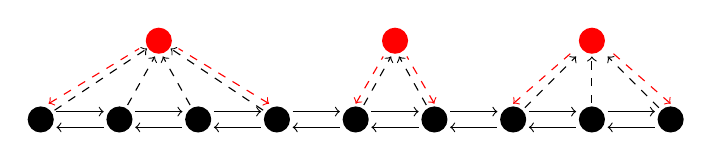
\begin{tikzpicture}
	\draw (1.5,1) node[circle, fill=red]{} ;
	\draw (0,0) node[circle, fill=black]{} ;
	\draw (1,0) node[circle, fill=black]{} ;
	\draw (2,0) node[circle, fill=black]{} ;
	\draw (3,0) node[circle, fill=black]{} ;

	\draw [->,dashed] (0,0) -- (1.35,0.9) ;
	\draw [->,dashed] (1,0) -- (1.45,0.8) ;
	\draw [->,dashed] (2,0) -- (1.55,0.8) ;
	\draw [->,dashed] (3,0) -- (1.65,0.9) ;

	\draw [<-,dashed,red] (0.1,0.2) -- (1.25,0.9) ;
	\draw [<-,dashed,red] (2.9,0.2) -- (1.75,0.9) ;

	\draw (4.5,1) node[circle, fill=red]{} ;
	\draw (4,0) node[circle, fill=black]{} ;
	\draw (5,0) node[circle, fill=black]{} ;

	\draw [->,dashed] (4,0) -- (4.45,0.8) ;
	\draw [->,dashed] (5,0) -- (4.55,0.8) ;

	\draw [<-,dashed,red] (4,0.2) -- (4.35,0.8) ;
	\draw [<-,dashed,red] (5,0.2) -- (4.65,0.8) ;

	\draw (7,1) node[circle, fill=red]{} ;
	\draw (6,0) node[circle, fill=black]{} ;
	\draw (7,0) node[circle, fill=black]{} ;
	\draw (8,0) node[circle, fill=black]{} ;

	\draw [->,dashed] (6,0) -- (6.8,0.8) ;
	\draw [->,dashed] (7,0) -- (7,0.8) ;
	\draw [->,dashed] (8,0) -- (7.2,0.8) ;

	\draw [<-,dashed,red] (6,0.2) -- (6.8,0.9) ;
	\draw [<-,dashed,red] (8,0.2) -- (7.2,0.9) ;


	\draw [->] (0.2,0.1) -- (0.8,0.1) ;
	\draw [->] (1.2,0.1) -- (1.8,0.1) ;
	\draw [->] (2.2,0.1) -- (2.8,0.1) ;
	\draw [->] (3.2,0.1) -- (3.8,0.1) ;
	\draw [->] (4.2,0.1) -- (4.8,0.1) ;
	\draw [->] (5.2,0.1) -- (5.8,0.1) ;
	\draw [->] (6.2,0.1) -- (6.8,0.1) ;
	\draw [->] (7.2,0.1) -- (7.8,0.1) ;

	\draw [<-] (0.2,-0.1) -- (0.8,-0.1) ;
	\draw [<-] (1.2,-0.1) -- (1.8,-0.1) ;
	\draw [<-] (2.2,-0.1) -- (2.8,-0.1) ;
	\draw [<-] (3.2,-0.1) -- (3.8,-0.1) ;
	\draw [<-] (4.2,-0.1) -- (4.8,-0.1) ;
	\draw [<-] (5.2,-0.1) -- (5.8,-0.1) ;
	\draw [<-] (6.2,-0.1) -- (6.8,-0.1) ;
	\draw [<-] (7.2,-0.1) -- (7.8,-0.1) ;


    \end{tikzpicture}
    \end{center}

\end{frame} 

\begin{frame}\frametitle{Some remarks}
    \begin{block}{Complexity}
	\begin{itemize}
	    \item Each step is $O(deg_{v})$
            \item Thus, LexBFS is linear
	    \item co-LexBFS is linear
	\end{itemize}
    \end{block}
    \begin{alertblock}{LexDFS}
	As of 2019, no known linear-time for LexDFS
    \end{alertblock}
\end{frame}

\begin{frame}\frametitle{Chordal Graph}

\begin{columns}[T] % align columns
\begin{column}{.48\textwidth}

	\begin{block}{Chordal Graph}
		A graph is chordal if all cycles of four or more vertices have an edge that is not part of the cycle but connects two of its vertices.
	\end{block}

\end{column}%
\hfill%
\begin{column}{.48\textwidth}

	\begin{block}{Perfect Elimination Ordering (=PEO)}
	$\sigma$ is a PEO if for each vertex v, v and its neighbours occuring after v in $\sigma$ form a clique.
	\end{block}

	\begin{block}{Chordal Graph}
		A graph is chordal if it admits a perfect elimination ordering.
	\end{block}
\end{column}
\end{columns}
\end{frame}


\begin{frame}\frametitle{Finding a Perfect Elimination Ordering}
	\begin{block}{Main Theorem}
		If G is chordal, any LexBFS ordering taken backward is a PEO.
	\end{block}

	\textbf{Proof:}

	c : non simplicial vertex

	Thus $\exists a <_{\sigma} b \in N(c)\text{ with }ab \notin E$

	$\sigma$ is a LexBFS thus $\exists d <_{\sigma} a\text{ with }db \in E, dc \notin E$

	$G$ is chordal, so $ad \notin E$
\end{frame}

\begin{frame}\frametitle{Ending the proof}

    \begin{center}
    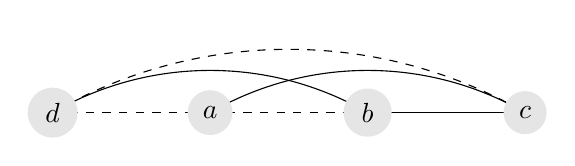
\begin{tikzpicture}
	\draw [dashed] (0,0) arc (120:60:6) ;
	\draw (0,0) arc (120:60:4) ;
	\draw (2,0) arc (120:60:4) ;
	\draw [dashed] (0,0) -- (2,0) ;
	\draw [dashed] (2,0) -- (4,0);
	\draw (4,0) -- (6,0) ;

	\draw (0,0) node[circle, fill=gray!20]{$d$} ;
	\draw (2,0) node[circle, fill=gray!20]{$a$} ;
	\draw (4,0) node[circle, fill=gray!20]{$b$} ;
	\draw (6,0) node[circle, fill=gray!20]{$c$} ;
    \end{tikzpicture}
    \end{center}

    \begin{itemize}
	\item \textbf{Initialization:} $(d, a, b)$ such that $da \notin E, ab \notin E, db \in E$
	\item \textbf{General Case:} $\exists d' <_{\sigma} d\text{ with }d'a \in E, d'b \notin E\text{ so }d'd \notin E$.
	\item Using the triple $(d', d, a)$, infinite chain.
    \end{itemize}

\end{frame}


\begin{frame}\frametitle{Some remarks}
     \begin{block}{Perfect Elimination co-Ordering is free}
	  With our implementation, co-PEO is linear on co-chordal.
     \end{block}


     \begin{alertblock}{Chordal Recognition}
	  For chordal recognition, need to verify if a given ordering is a PEO.
     \end{alertblock}
\end{frame}


\begin{frame}[fragile]\frametitle{Verify if an ordering is a PEO}
    \begin{lstlisting}[language = Python]
    for x in vertices:
	RN[x] = neighborstotheright(x)
	parent[x] = leftmost(RN[x])
    T = treefrompointers(parent)
    for x in T in postorder:
	if (RN[x] \ x) not included in RN[parent[x]]:
	    return False
    return True
    \end{lstlisting}
    
    \begin{block}{Corollary}
	Recognizing chordal graphs can be done in linear time.
    \end{block}
\end{frame}

\begin{frame}[fragile]\frametitle{Easily adaptable for co-chordal}
    Easily adapted for running on the complementary :
	\begin{itemize}
	     \item parent[x] = leftmost non-neighbor to the right of x
             \item check if RN[parent[x]] is included in RN[x]
	\end{itemize}

    \begin{block}{Corollary}
	Recognizing co-chordal graphs can be done in linear time.
    \end{block}
\end{frame}

\end{document}
